\documentclass[14pt]{extbook}
\usepackage{multicol, enumerate, enumitem, hyperref, color, soul, setspace, parskip, fancyhdr} %General Packages
\usepackage{amssymb, amsthm, amsmath, latexsym, units, mathtools} %Math Packages
\everymath{\displaystyle} %All math in Display Style
% Packages with additional options
\usepackage[headsep=0.5cm,headheight=12pt, left=1 in,right= 1 in,top= 1 in,bottom= 1 in]{geometry}
\usepackage[usenames,dvipsnames]{xcolor}
\usepackage{dashrule}  % Package to use the command below to create lines between items
\newcommand{\litem}[1]{\item#1\hspace*{-1cm}\rule{\textwidth}{0.4pt}}
\pagestyle{fancy}
\lhead{Progress Quiz 10}
\chead{}
\rhead{Version C}
\lfoot{5170-5105}
\cfoot{}
\rfoot{Summer C 2021}
\begin{document}

\begin{enumerate}
\litem{
Choose the graph of the equation below.\[ f(x) = \sqrt[3]{x + 10} + 5 \]\begin{enumerate}[label=\Alph*.]
\begin{multicols}{2}\item 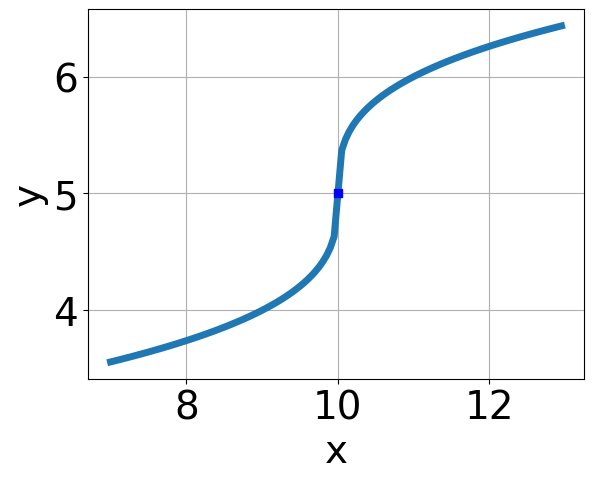
\includegraphics[width = 0.3\textwidth]{../Figures/radicalEquationToGraphAC.png}\item 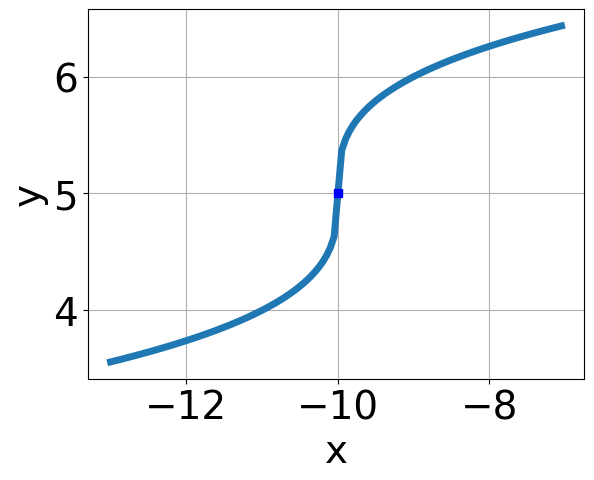
\includegraphics[width = 0.3\textwidth]{../Figures/radicalEquationToGraphBC.png}\item 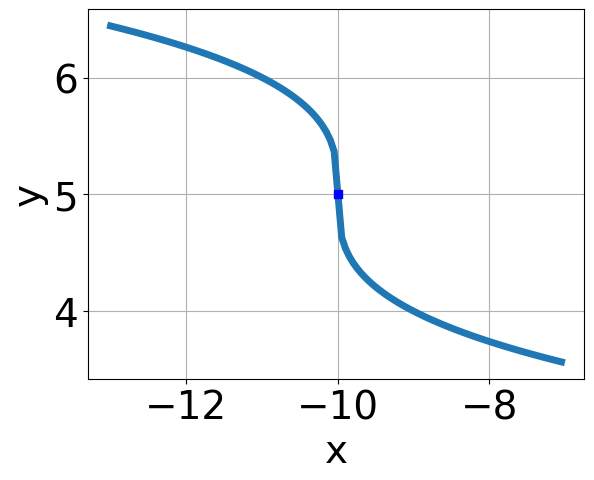
\includegraphics[width = 0.3\textwidth]{../Figures/radicalEquationToGraphCC.png}\item 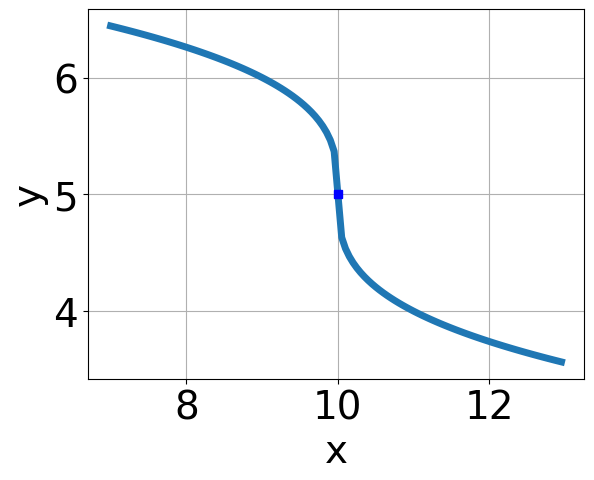
\includegraphics[width = 0.3\textwidth]{../Figures/radicalEquationToGraphDC.png}\end{multicols}\item None of the above.
\end{enumerate} }
\litem{
Solve the radical equation below. Then, choose the interval(s) that the solution(s) belongs to.\[ \sqrt{-32 x^2 - 56} - \sqrt{88 x} = 0 \]\begin{enumerate}[label=\Alph*.]
\item \( x_1 \in [-2.57, -1.51] \text{ and } x_2 \in [-2.7,0.5] \)
\item \( x \in [-1.08,-0.6] \)
\item \( \text{All solutions lead to invalid or complex values in the equation.} \)
\item \( x_1 \in [0.74, 2.1] \text{ and } x_2 \in [-0.2,3.2] \)
\item \( x \in [-2.57,-1.51] \)

\end{enumerate} }
\litem{
Choose the equation of the function graphed below.
\begin{center}
    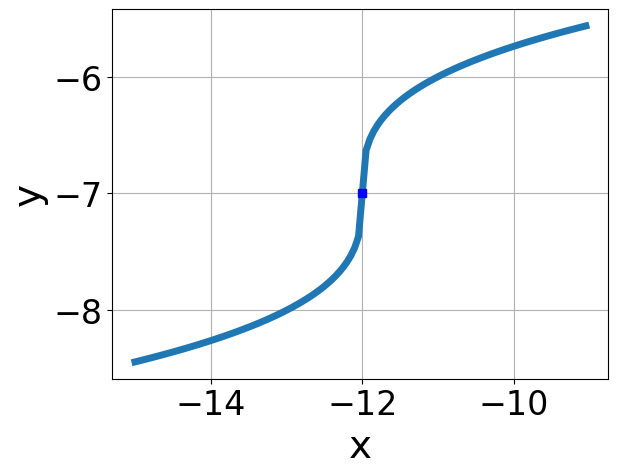
\includegraphics[width=0.5\textwidth]{../Figures/radicalGraphToEquationC.png}
\end{center}
\begin{enumerate}[label=\Alph*.]
\item \( f(x) = \sqrt[3]{x - 12} - 7 \)
\item \( f(x) = - \sqrt[3]{x - 12} - 7 \)
\item \( f(x) = \sqrt[3]{x + 12} - 7 \)
\item \( f(x) = - \sqrt[3]{x + 12} - 7 \)
\item \( \text{None of the above} \)

\end{enumerate} }
\litem{
Choose the graph of the equation below.\[ f(x) = - \sqrt[3]{x - 10} - 4 \]\begin{enumerate}[label=\Alph*.]
\begin{multicols}{2}\item 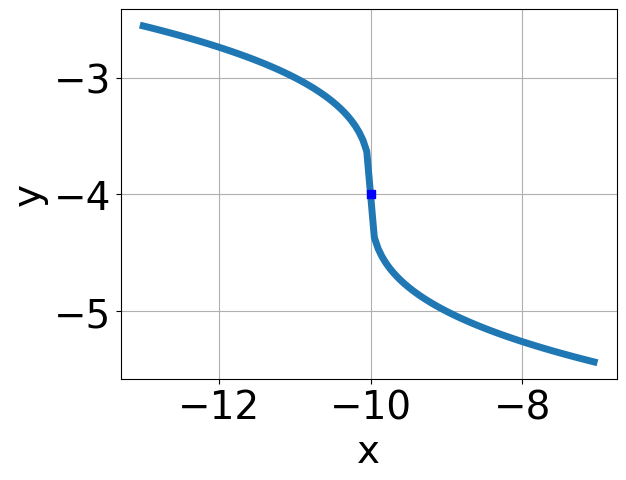
\includegraphics[width = 0.3\textwidth]{../Figures/radicalEquationToGraphCopyAC.png}\item 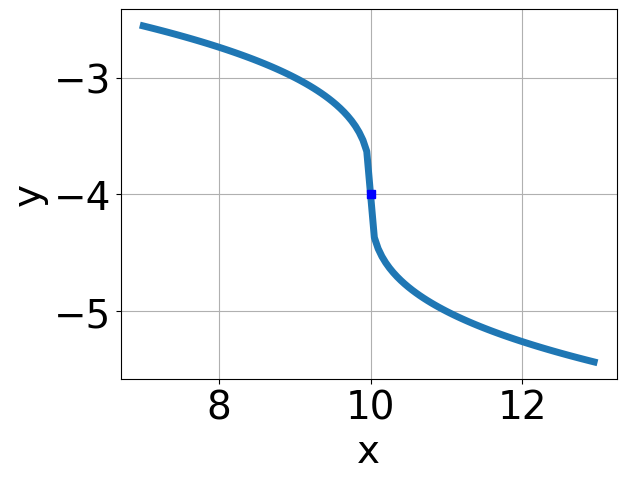
\includegraphics[width = 0.3\textwidth]{../Figures/radicalEquationToGraphCopyBC.png}\item 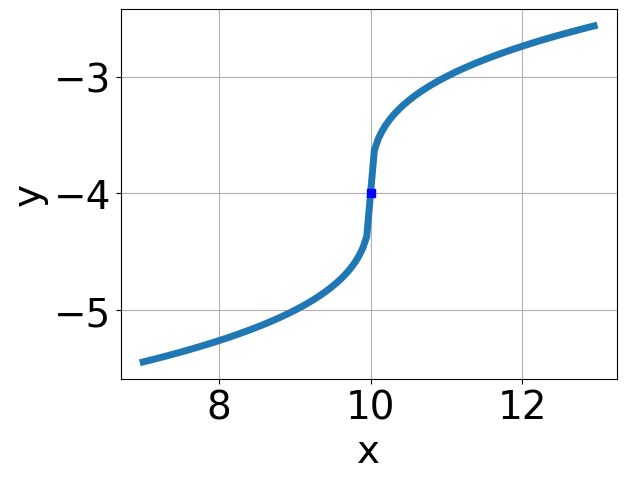
\includegraphics[width = 0.3\textwidth]{../Figures/radicalEquationToGraphCopyCC.png}\item 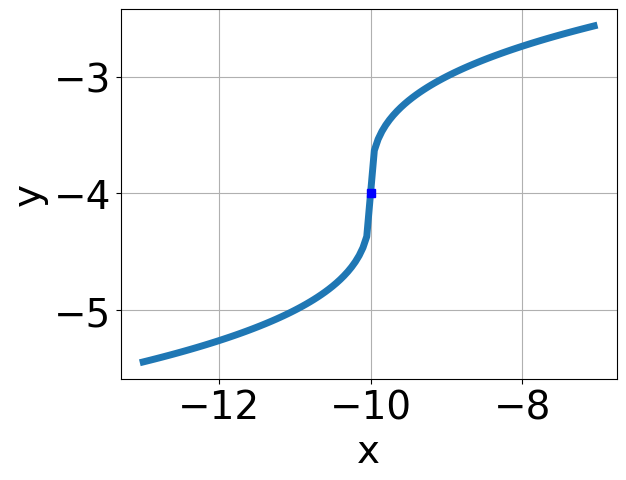
\includegraphics[width = 0.3\textwidth]{../Figures/radicalEquationToGraphCopyDC.png}\end{multicols}\item None of the above.
\end{enumerate} }
\litem{
What is the domain of the function below?\[ f(x) = \sqrt[8]{3 x + 8} \]\begin{enumerate}[label=\Alph*.]
\item \( (-\infty, a], \text{where } a \in [-0.38, 1.62] \)
\item \( [a, \infty), \text{ where } a \in [-3.1, -1.8] \)
\item \( [a, \infty), \text{where } a \in [-0.7, 0.7] \)
\item \( (-\infty, a], \text{where } a \in [-8.67, -1.67] \)
\item \( (-\infty, \infty) \)

\end{enumerate} }
\litem{
Solve the radical equation below. Then, choose the interval(s) that the solution(s) belongs to.\[ \sqrt{4 x + 5} - \sqrt{6 x + 3} = 0 \]\begin{enumerate}[label=\Alph*.]
\item \( x \in [2.5,4.7] \)
\item \( x_1 \in [-1.8, -0.8] \text{ and } x_2 \in [1,3] \)
\item \( x_1 \in [-1.8, -0.8] \text{ and } x_2 \in [-1.5,0.5] \)
\item \( x \in [-0.6,2] \)
\item \( \text{All solutions lead to invalid or complex values in the equation.} \)

\end{enumerate} }
\litem{
Solve the radical equation below. Then, choose the interval(s) that the solution(s) belongs to.\[ \sqrt{3 x + 9} - \sqrt{5 x - 9} = 0 \]\begin{enumerate}[label=\Alph*.]
\item \( x \in [6,11] \)
\item \( \text{All solutions lead to invalid or complex values in the equation.} \)
\item \( x_1 \in [-5, -1] \text{ and } x_2 \in [0.8,3.8] \)
\item \( x_1 \in [-5, -1] \text{ and } x_2 \in [5,14] \)
\item \( x \in [-2,5] \)

\end{enumerate} }
\litem{
What is the domain of the function below?\[ f(x) = \sqrt[8]{8 x + 6} \]\begin{enumerate}[label=\Alph*.]
\item \( [a, \infty), \text{where } a \in [-1.77, -1.02] \)
\item \( [a, \infty), \text{ where } a \in [-1.06, -0.68] \)
\item \( (-\infty, \infty) \)
\item \( (-\infty, a], \text{where } a \in [-1.91, -1.11] \)
\item \( (-\infty, a], \text{where } a \in [-1.07, -0.23] \)

\end{enumerate} }
\litem{
Choose the equation of the function graphed below.
\begin{center}
    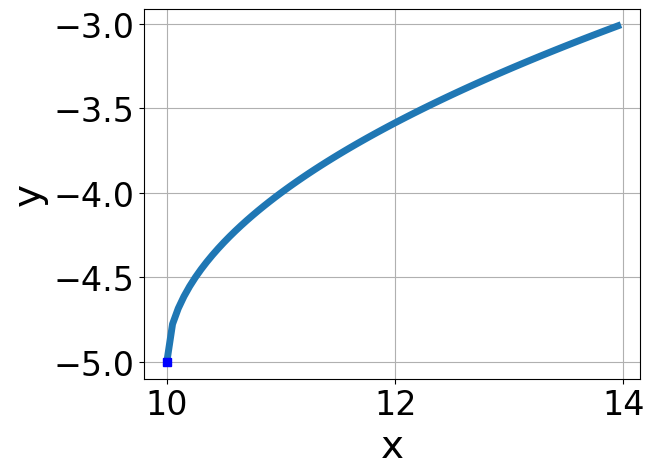
\includegraphics[width=0.5\textwidth]{../Figures/radicalGraphToEquationCopyC.png}
\end{center}
\begin{enumerate}[label=\Alph*.]
\item \( f(x) = \sqrt{x - 10} - 5 \)
\item \( f(x) = - \sqrt{x - 10} - 5 \)
\item \( f(x) = \sqrt{x + 10} - 5 \)
\item \( f(x) = - \sqrt{x + 10} - 5 \)
\item \( \text{None of the above} \)

\end{enumerate} }
\litem{
Solve the radical equation below. Then, choose the interval(s) that the solution(s) belongs to.\[ \sqrt{-6 x^2 + 48} - \sqrt{12 x} = 0 \]\begin{enumerate}[label=\Alph*.]
\item \( x_1 \in [-1, 11] \text{ and } x_2 \in [3.4,5.9] \)
\item \( \text{All solutions lead to invalid or complex values in the equation.} \)
\item \( x_1 \in [-6, 0] \text{ and } x_2 \in [1.7,3.1] \)
\item \( x \in [-6,0] \)
\item \( x \in [-1,11] \)

\end{enumerate} }
\end{enumerate}

\end{document}